\documentclass{article}
\usepackage{graphicx} 
\usepackage[utf8]{inputenc}
\usepackage{amsmath, amsfonts, amssymb, bm}
\usepackage{graphicx, geometry, wrapfig, float, multicol, mathtools, array, csquotes, lscape, setspace}
\usepackage[dvipsnames]{xcolor}
\usepackage[export]{adjustbox}
\usepackage{tikz}
\usepackage[most]{tcolorbox}
\usetikzlibrary{positioning, fit}
\usepackage{multirow, booktabs, makecell, diagbox, cancel}
\usepackage{soul}
\usepackage{hyperref}
\usepackage{xstring}
\usepackage{txfonts}

\newcommand{\drawback}{\textbf{\textcolor{Red}{drawback }}}
\newcommand{\advantage}{\textbf{\textcolor{Green}{advantage }}}

\hypersetup{
    colorlinks=true,
    allcolors=.,
    pdftitle={Explainable AI Notes},
    linkcolor=black
    }
\geometry{
    top=3.5cm,
    bottom=3.0cm,
    outer=1.0cm,
    inner=2.0cm
}
\newcommand{\red}{\color{red}}
\newcommand{\blue}{\color{blue}}
\newcommand{\black}{\color{black}}
% Required for inserting images
\setlength{\parindent}{0mm}
\DeclareMathOperator{\EX}{\mathbb{E}}% expected value
\newcommand{\HRule}[1]{\rule{\linewidth}{#1}}
\renewcommand{\ref}[1]{\textbf{\ref{#1}}}

\begin{document}
\title{ \normalsize \textsc{}
		\\ [2.0cm]
		\HRule{1.5pt} \\
		\LARGE \textbf{\uppercase{Explainable AI}
		\HRule{2.0pt} \\ [0.6cm] \LARGE{Academic Year: 2023/2024} \vspace*{10\baselineskip}}
		}

\author{\textbf{Author} \\ 
    Lorenzo Bonanni\\
    lorenzo.bonanni@studenti.univr.it}

\maketitle
\newpage
\tableofcontents

\part{Introduction \& Motivation}
AI (and particularly ML) can solve very complex problems in real life such as: Autonomous vehicles, Industrial automation and robotics Medical imaging and diagnosis ecc..
The problem with most of the ML models is that they are black boxs i.e we cannot understand the motivation behind the output.\\

The goal of Explainable AI (XAI) is to explain the behaviour of AI systems, in order to increase the
level of understanding and \emph{trust}. 
\begin{figure}[H]
    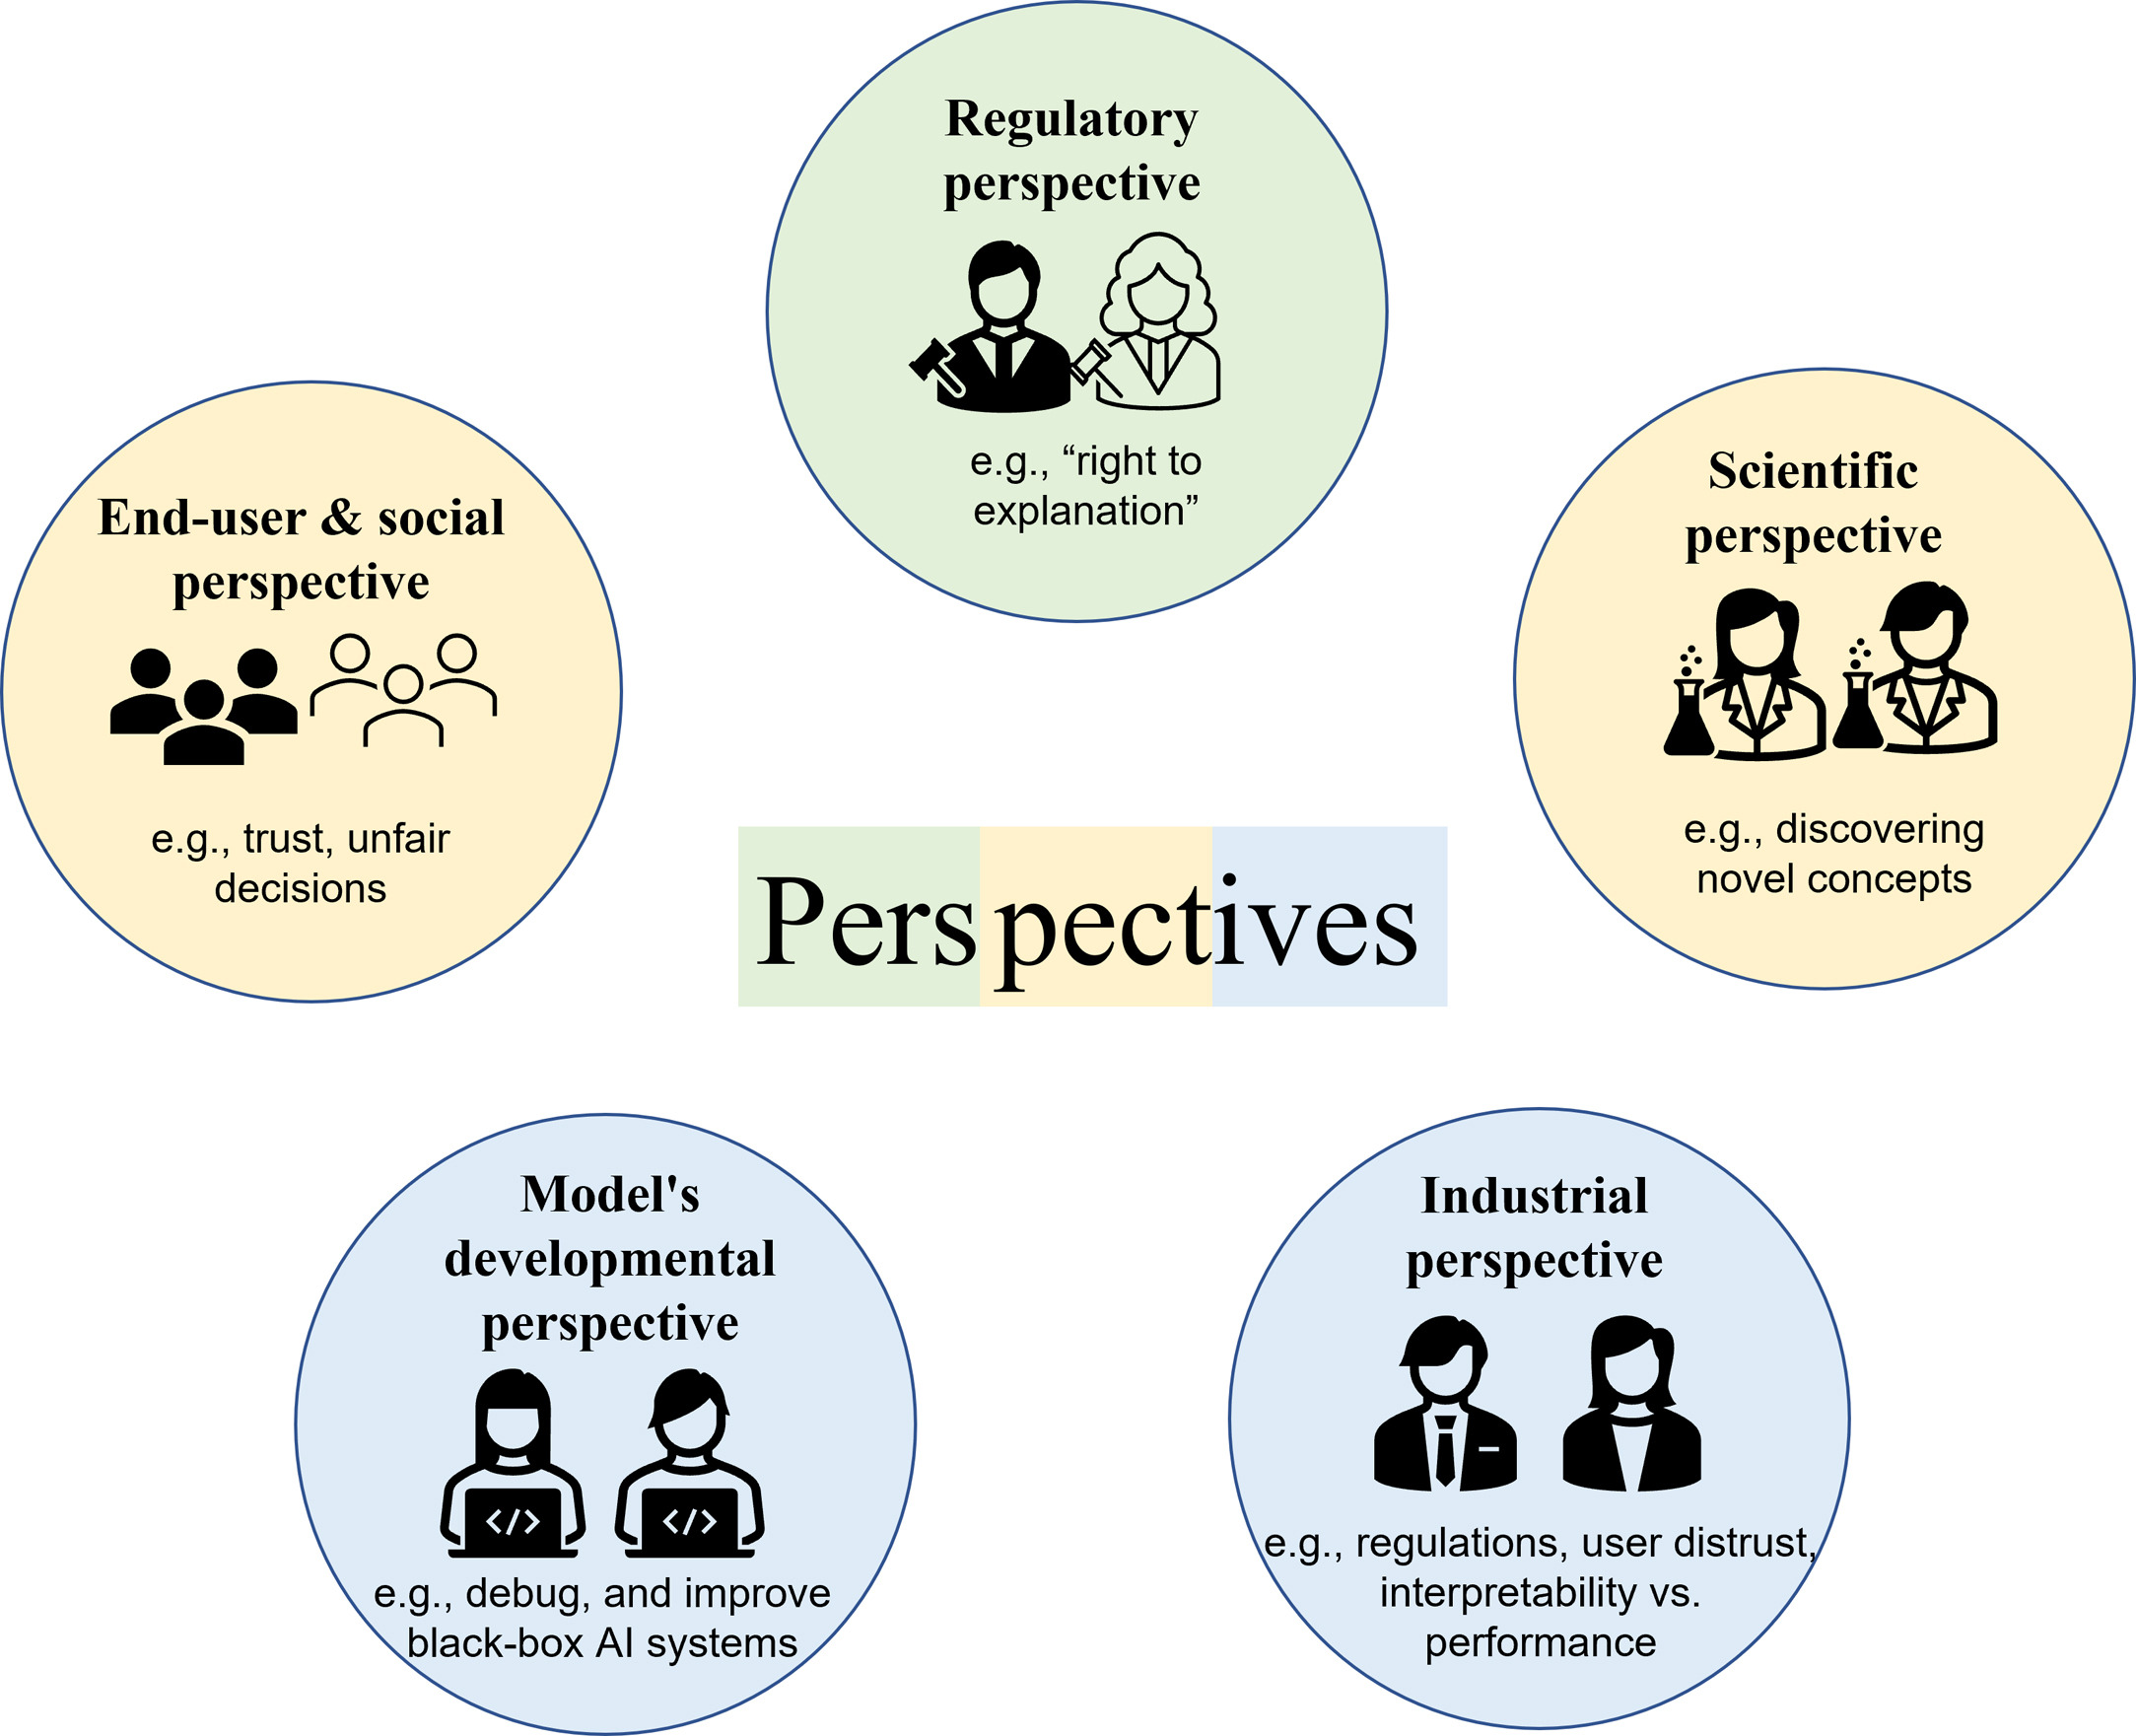
\includegraphics[width=0.5\textwidth]{img/motivation.jpg}
    \centering
    \caption{Summary of the main motivations regarding the use of XAI}
\end{figure}
We can summarize the motivation into 5 main points:
\begin{enumerate}
    \item Regulatory Perspective
    \item Scientific Perspective
    \item Industrial Perspective
    \item Model's developmental perspective
    \item End-user and social perspective
\end{enumerate}
\section{Motivation}
\subsection*{Regulatory Perspective}
Black-box AI systems are being utilized in many areas of our daily lives, which could be resulting in unacceptable decisions, especially those that may lead to legal effects. 
The European Union's General Data Protection Regulation (GDPR)\footnote{\url{https://www.privacy-regulation.eu/en/r71.htm}} is an example of why XAI is needed from a regulatory perspective. 
These regulations create what is called the \emph{right to explanation}, by which a user is entitled to request an explanation about the decision made by the algorithm that considerably influences them.

\subsection*{Scientific Perspective}
When building black-box AI models, we aim to develop an approximate function to address the given problem. 
Therefore, after creating the black-box AI model, the created model represents the basis of knowledge, rather than the data. 
Based on that, XAI can be helpful to reveal the scientific knowledge extracted by the black-box AI models, which could lead to discovering novel
concepts in various branches of science.

\subsection*{Industrial perspective}
Regulations and user distrust in black-box AI systems represent challenges to the industry in applying complex and accurate 
black-box AI systems. Less accurate models that are more interpretable may be preferred in the industry because of regulation
reasons. A major advantage of XAI is that it can help in mitigating the common trade-off between model interpretability and performance,
thus meeting these common challenges. 
However, it can increase development and deployment costs.

\subsection*{Model's developmental perspective}
Several reasons could contribute to inappropriate results for black-box AI systems, such as limited training data, biased training data, outliers, adversarial data, and model overfitting. 
Therefore, what black-box AI systems have learned and why they make decisions need to be understood, primarily when they affect humans lives. 
For that, the aim will be to use XAI to understand, debug, and improve the black-box AI system to enhance its robustness, increase safety and user trust, and minimize or prevent faulty behavior, bias, unfairness, and discrimination.

\subsection*{End-user and social perspective}
In the literature of deep learning, it has been shown that altering an image such that humans cannot observe the change can lead the model in producing a wrong class label (Adversarial Attacks). 
On the contrary, completely unrecognizable images to humans can be recognizable with high confidence using DL models.
Such findings could raise doubts about trusting such black-box AI models. 
The possibility to produce unfair decisions is another concern about black-box AI systems. 
This could happen in case black-box AI systems are developed using data that may exhibit human biases and prejudices.
Therefore, producing explanations and enhancing the interpretability of the black-box AI systems will help in increasing trust because it will be possible to understand the rationale behind the model's decisions, and we can know if
the system serves what it is designed for instead of what it was trained for. Furthermore, the demand for the fairness of black-box AI systems decisions, which cannot be ensured by error measures, often leads to the need for
interpretable models.

% \part{title}
\section{XAI - One topic, two keywords}
\begin{minipage}[c]{0.3\textwidth}
    \begin{figure}[H]
        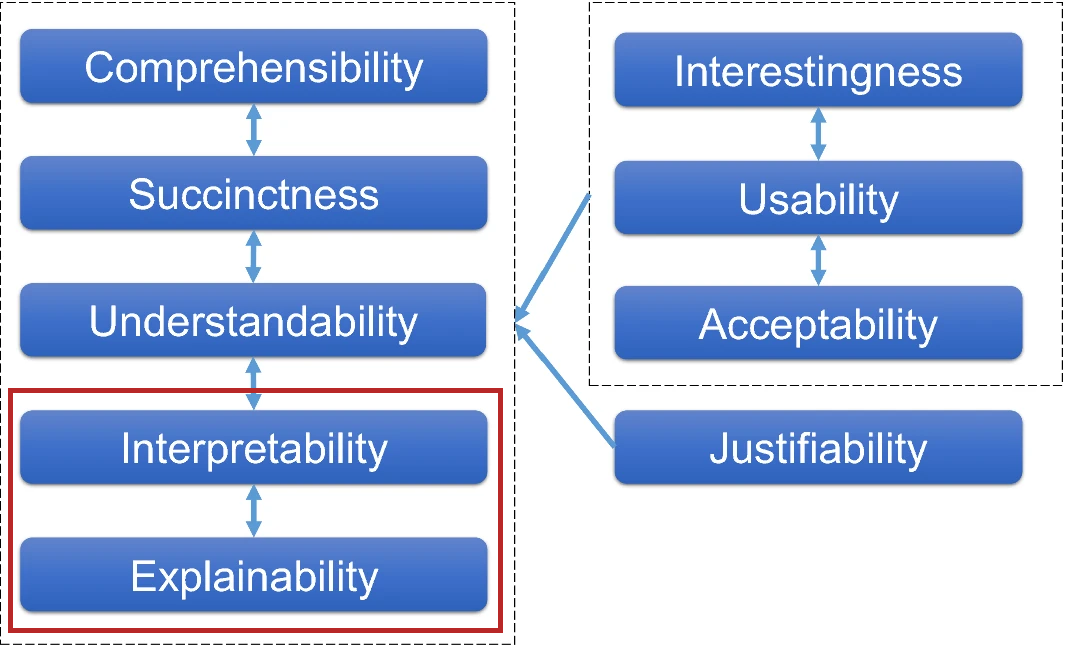
\includegraphics[width=\textwidth]{img/many_words.png}
        \centering
        \caption{Outline of the relationships between the common XAI terminologies}
    \end{figure}    
\end{minipage}
\hfill%
\begin{minipage}[c]{0.65\textwidth}
    In the Explainable AI domains there many terms that seems to be the same meaning.
    Specifically we are interested into two terms: Explainablility and Interpretability.\\
    
    Explainablility provide insights about an AI model while Interpretability tells if the insights make sense to the audience.
\end{minipage}

\section{Types of XAI}
\begin{minipage}[c]{0.5\textwidth}
    \begin{figure}[H]
        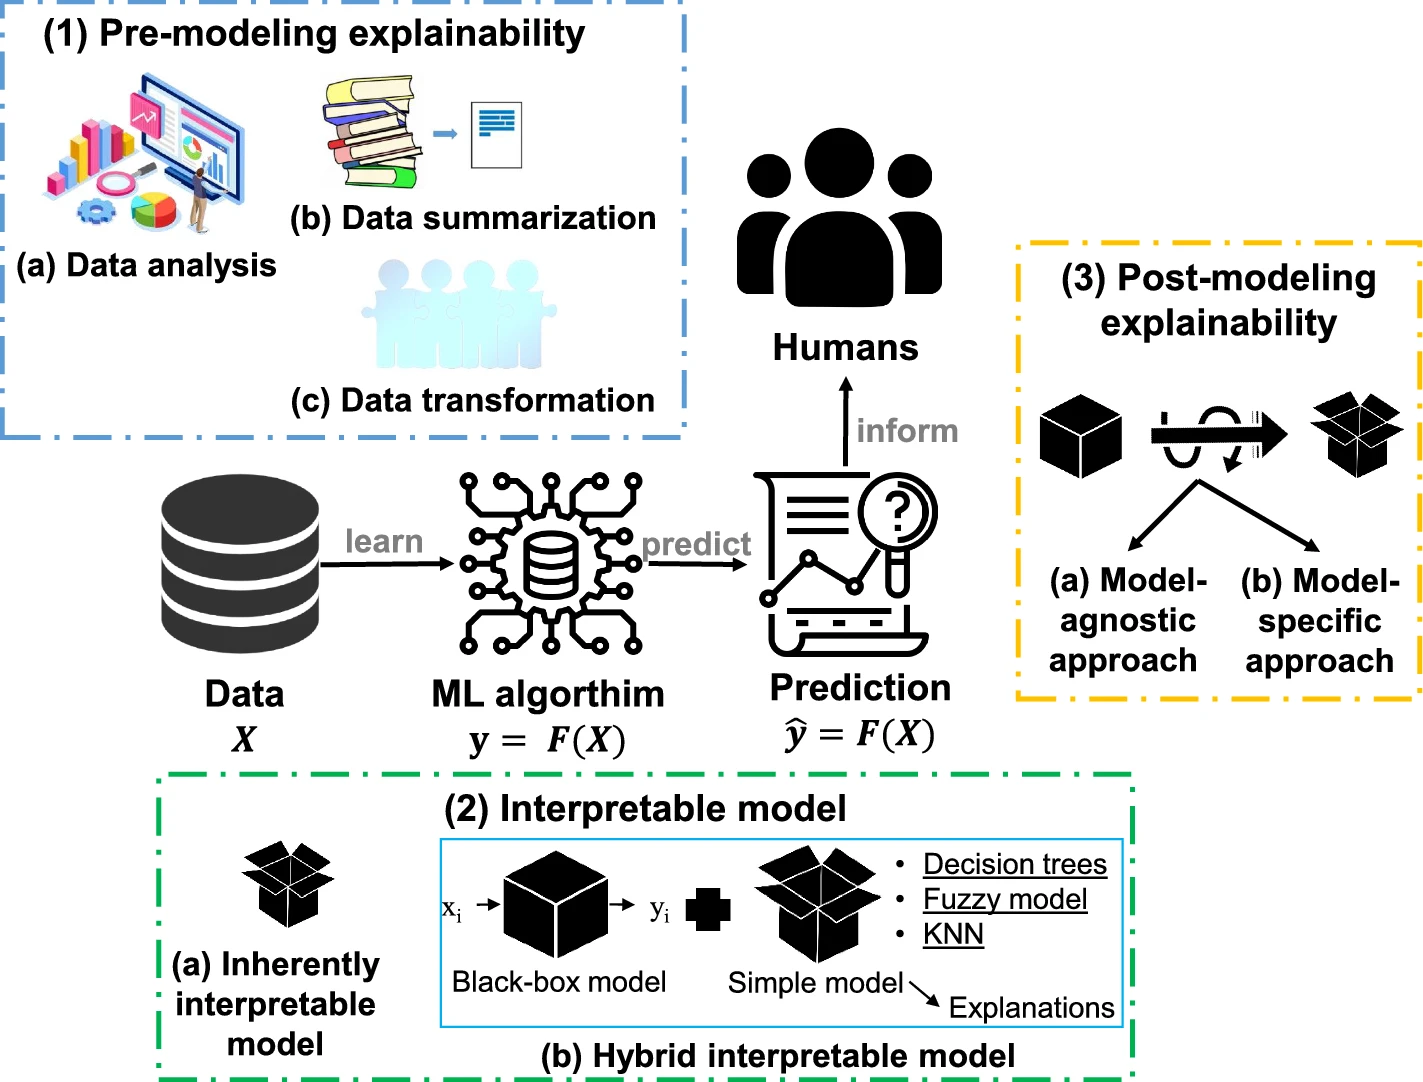
\includegraphics[width=0.8\textwidth]{img/types_XAI.png}
        \centering
        \caption{Outline of the relationships between the common XAI terminologies}
    \end{figure}
\end{minipage}
\begin{minipage}[c]{0.5\textwidth}
    There are three main types of Explainablility:
    \begin{enumerate}
        \item \textbf{Pre-modeling explainability}: summarize input data to identify most relevant features or aspects, based on statistical analysis. Some examples are: K-Means and PCA
        \item \textbf{Post-modeling explainability}: explain the results of a black-box model. Some tecniques include: 
        \begin{itemize}
            \item \emph{Feature relevance}: which input data mostly influences the output?
            \item \emph{Simplification}: aims to make a simplified version of the original model that has an
            optimized function, significantly reduces the complexity, has a simpler implementation
            process, and performance is comparable to the original version.
            \item \emph{Visualization}: interprets a models behavior by visual representations. Visualiza-
            tion techniques are considered the best way to explain the complicated inner interac-
            tions of the variables of the model, and they can be combined with other methods in
            order to increase their interpretability ability.
            \item \emph{Textual justifications}: explains a model by generating explanations in the form of
            text
            \item \emph{Contrastive explanations}: clarifies why an event occurred in contrast to another
        \end{itemize}
        \item \textbf{Interpretable models}: the model is not black-box on its own. some examples include: Linear or logistic regression and Decision trees
    \end{enumerate}
\end{minipage}\\

There are three main properties for interpretability:
\begin{itemize}
    \item Algorithmic transparency: The model can be expressed as a set of known mathematical or logical relations
    \item Decomposability: The model can be decomposed in submodules, with clear indication of connections between them
    \item Simulatability: The model can be easily simulated by a human, given only any input
\end{itemize}
\section{Causal analysis \& discovery}
Reconstructing the \textbf{causal relations} behind the phenomena we observe is 
a fundamental problem in all fields of science.
The traditional approach is to conduct active experiments, but in many fields
manipulations of the complex system under study are either impossible, 
unethical, or very expensive.
On the other hand, modern science generates an ever-growing amount of data 
from these systems, in particular time series data.
Concurrently, novel computing hardware today allows efficient processing 
of massive amounts of data. These developments have led to emerging interest 
in the problem of reconstructing causal networks or causal discovery from 
observational time series.\\

The definition of causality is that $X \rightarrow Y$ if and only if an intervention or
manipulation in $X$ has an effect on $Y$.
A practical example could be the altitude and the temperature as in Figure \ref{fig:tempvsheight}.
As the height increases the temperature lowers.

\begin{minipage}[c]{0.3\textwidth}
    \begin{figure}[H]
        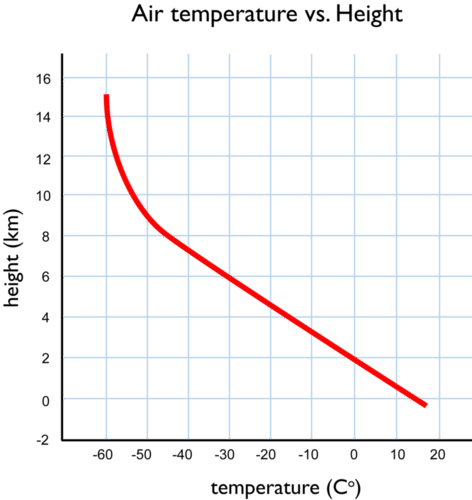
\includegraphics[width=0.6\textwidth]{img/tempvsheight.png}
        \centering
        \caption{Varion of temperature with respect to the height}
        \label{fig:tempvsheight}
    \end{figure}
\end{minipage}
\begin{minipage}[c]{0.6\textwidth}
    One of the main motivations behind causal analysis is a property called \textbf{similability}, 
    the ability o easily predict the output, given only any possible input.
\end{minipage}\\


We will consider causal analysis and discovery for time series since typically, 
input and output of a system are temporal signals, and we are interested in understanding 
how the system evolves and behaves over time.
This means, we want to understand how the temporal evolution of the output signal is affected
by the input signal (\textbf{and discovering which one is the input}).
We will denote as $V_T$ a variable $V$ which is observed for a temporal horizon $T$ (either continuous or
discrete)
\subsection{Structural causal model}
\begin{equation}
    V_t^j \coloneqq \textcolor{red}{f^j}(\textcolor{blue}{pa(V^j_t)}, \eta^j_t)\quad\text{for all }V_t^j\in \bm{V_t} \text{ and } t\in\mathbb{Z}
\end{equation}
Where $\textcolor{red}{f^j}$ is a generic non linear function, $\textcolor{blue}{pa(V^j_t)}$ are the parents of the variable $V^j$ i.e its causes and
$\eta^j_t$ is noise which comes from the uncertanty of the model or of the measurements.
\subsection{Granger's definition of causality (1969)}\label{sec:granger}
Given (temporal) variables $X$ and $Y$, we say that $X\;Granger-causes\;Y$
if $X$ contains information which affects $Y$ at time t, and such
information is not contained in the past of the universe ($Y$'s past or
other variables'past). In other words $Y$ depens \textbf{only} on $X$ and no other variables.If we only consider $Y$, we refer to bivariate causality \\

Granger's definition can be written in the following way as an autoregressive process:
\begin{equation}
    \bm{x_t}=\sum_{\tau=1}^{\tau_{max}}\phi(\tau)\bm{x}_{t-\tau}+\eta_t
\end{equation}
This formulation implies causality in mean (autoregressive model), this 
is a problem since it does not capture information about the distribution of the data.

\subsection{Conditional Mutual Information}
A more general definition comes from Schreibe: (bivariate) transfer entropy
\begin{equation}
    I^{TEbiv}_{X\rightarrow Y}=I(X_t^-;Y_t|Y_t^-)
    \label{eq:tebiv}
\end{equation}
where the `-` indicates the past of the variable and $I(X;Y|Z)$ denotes the Conditional Mutual Information (CMI).

\begin{equation}
    I(X;Y|Z)=\iiint{p(x,y,z)\log_2{\frac{p(x, y| z)}{p(x|z)\cdot p(y|z)}}dx\;dy\;dz}
    \label{eq:cmi}
\end{equation}
CMI (also called Related Entropy) comes from the concept of KL(Kullback-Leibler) divergence.
\begin{equation}
    D(p||q)=\sum_{x\in\mathcal{X}}p(x)\log{\frac{p(x)}{q(x)}}
\end{equation}
The KL divergence measures the degree of similarity (the distance) between two distribution namely $p$ and $q$.\\

The equation for the KL divergence seems to come out of the air, but in reality the equation is really simple...

We have two pieces, the first $\frac{p(x)}{q(x)}$ measures the distance between 
the distribution $p$ and the distribution $q$, then we add the $log$, we do that 
because if $p(x)=q(x)$ (i.e they are the same distribution) then the division will 
be 1. Since they are the same distribution the distance between the distributions should be 0 but for now it is only 1. 
If we add the $log$ then $\log(1)=0$ and so the distance is 0. The second piece $p(x)$ is a weight, this 
is used because we want to weight the distance based on the likelihood of the input
 $x$, this mean that we care less of high distance if the input is unlikely.
I've omitted a small detail, I've talked about distance between distributions 
but in reality what I meant was distance between points(e.g $p(x)$) in the 
distributions and so we need to add a summation to the equation 
(or an integral in case of continuous distributions) so to add the contribution
 of each individual point.\\

Similarly Mutual Information (MI) measures the \textbf{discrepancy} between \textbf{joint distribution} (p(x,y)) and the \textbf{product} (p(x)p(y)) of individual distributions.
Mutual Information(MI) is the same as CMI (eq \ref{eq:cmi}) but without the conditioning on $z$, so for the dicrete case the equation is:
\begin{equation}\label{eq:mi_disc}
    \begin{split}
        I(X;Y)&=\sum_{x\in\mathcal{X}}\sum_{y\in\mathcal{Y}}p(x,y)\cdot\log{\frac{p(x,y)}{p(x)p(y)}}\\
        &=D(p(x,y)||p(x)p(y))
    \end{split}
\end{equation}
This means that we can see MI as the KL divergence between the joint distribution and the product distribution.

\begin{tcolorbox}[colbacktitle=black!7!white,coltitle=black!75!white,title=\textbf{Statistics Recall}]
Let's make a quick statistics recall:\\
Given two random variables $x$ and $y$ if $x \text{ \textbf{indipendent}of } y$\\
$p(x,y) = p(x)p(y)$ so the product distribution is equal to the joint distribution\\\\
Given two random variables $x$ and $y$ if $x \text{ \textbf{dependent }on } y$\\
$p(x,y)=p(y)\cdot p(x|y)$
\end{tcolorbox}

So with MI we are trying to check if $x$ and $y$ are dependent:\\

\begin{center}
    \begin{minipage}[t]{0.4\textwidth}
        \noindent
        Assume $x$ and $y$ are \textit{\textbf{independent}}:
        \begin{equation}
            \begin{split}
                I(X;Y)&=\sum_{x\in\mathcal{X}}\sum_{y\in\mathcal{Y}}p(x,y)\cdot\log{\frac{\textcolor{red}{p(x,y)}}{p(x)p(y)}}\\
                &=\sum_{x\in\mathcal{X}}\sum_{y\in\mathcal{Y}}p(x,y)\cdot\log{\frac{\textcolor{red}{p(x)p(y)}}{p(x)p(y)}}\\
                &=\sum_{x\in\mathcal{X}}\sum_{y\in\mathcal{Y}}p(x,y)\cdot\log{\cancel{\frac{p(x)p(y)}{p(x)p(y)}}}\\
                &=\sum_{x\in\mathcal{X}}\sum_{y\in\mathcal{Y}}p(x,y)\cdot\log{1}\\
                &=\sum_{x\in\mathcal{X}}\sum_{y\in\mathcal{Y}}p(x,y)\cdot0\\
                &=0
            \end{split}
        \end{equation}
    \end{minipage}
    \begin{minipage}[t]{0.4\textwidth}
        \noindent
        Assume $x$ and $y$ are \textit{\textbf{dependent}}:
        \begin{equation}
            \begin{split}
                I(X;Y)&=\sum_{x\in\mathcal{X}}\sum_{y\in\mathcal{Y}}p(x,y)\cdot\log{\frac{\textcolor{red}{p(x,y)}}{p(x)p(y)}}\\
                &=\sum_{x\in\mathcal{X}}\sum_{y\in\mathcal{Y}}p(x,y)\cdot\log{\frac{\textcolor{red}{p(y)p(x|y)}}{p(x)p(y)}}\\
                &=\sum_{x\in\mathcal{X}}\sum_{y\in\mathcal{Y}}p(x,y)\cdot\log{\frac{\cancel{p(y)}p(x|y)}{p(x)\cancel{p(y)}}}\\
                &=\sum_{x\in\mathcal{X}}\sum_{y\in\mathcal{Y}}p(x,y)\cdot\log{\frac{p(x|y)}{p(x)}}\\
                &\ne 0
            \end{split}
        \end{equation}
    \end{minipage}
\end{center}
% \newpage
So to recap:
\begin{itemize}
    \item $x \text{ and } y$ DEPENDANT$\rightarrow\;MI\ne 0$
    \item $x \text{ and } y$ INDIPENDENT$\rightarrow\;MI=0$
\end{itemize}
CMI(Eq \ref{eq:cmi}) is essentially the same but we measure if two variables are dependent given that both are conditioned by a third variable.
In other words given $x,y \text{ and } z$ how much $x$ and $y$ are indipendent given that both depend on $z$.
Differently from Granger Causality (Section \ref{sec:granger}) in MI and CMI 
we are evaluating the entire distribution instead of only the mean so it is 
more informative.\\
Given the above definition we can generalize the Granger formulation to include CMI:\\
$I^{FullCI}_{i\rightarrow j}(\tau)=I(X^i_{t-\tau};X^j_t|\bm{X}_t^{(t-1,\ldots,t-\tau_{max})}\setminus\{X^i_{t-\tau}\})$ 
\\here $\bm{X}_t^{(t-1,\ldots,t-\tau_{max})}$ is what we called $Z$ before i.e the past of all the variables.\\

To better understand causasality we can visualize it as a graph:
\begin{figure}[H] \label{fig:causalgraph}
    \centering
    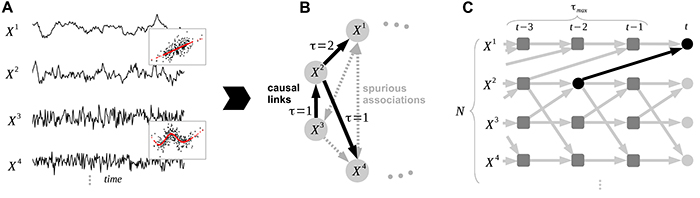
\includegraphics[width=0.8\textwidth]{img/visualization.jpeg}
    \caption{A time series dataset (panel A) from a complex system of which we try to reconstruct the underlying causal dependencies (panel B), 
    accounting for linear and nonlinear dependencies and including their time lags (link labels). }
\end{figure}
Figure \ref{fig:causalgraph}B represents the causal realation between variables, you can see solid and dashed lines.
The first represents a real causal relation between variables, while the second represent what's called a spurious association, 
this means that we find a relation between variables but those varibles are not related and this relation occurs either by chance 
or it is caused by a third unseed variable.\\\\
A simple example of this can be a causal graph representing the relation between the \emph{number of ice cream cones sold} in a city
per month and the \emph{number of sunburn cases} reported in the city per month.
If we analize that graph we can see that the number of ice cream cones sold in one month causes the number of sunburn cases reported in the next month.
Intuitively this relation does not make sense, how is it possible that an increase in number of ice creams sold causes the number of sunburs to raise?
In fact this relation is spurious since both are caused by a third variable, namely the \emph{average temperature} in the city per month.
Higher temperatures cause more people to buy ice cream and also expose themselves to the sun, leading to more sunburns.
As you can see in the picture on top of the edges there is written a number, it states the time lag difference in the relation, to make it more clear 
let's go back to the ice cream example. Assume $X^3$ is the number of ice cream sold and $X^2$ represents the number of sun burns.
As we said before the number of ice cream cones sold in one month causes the number of sunburn cases reported in the \textbf{next month}, 
here the key point is next month, as we can see in the graph is written as $\tau=1$ this means that $X^3_{t-1}\rightarrow X^2_{t}$, where the arrow represents the causal realtion.

% TODO: Figure \ref{fig:causalgraph}C

\subsection{Causal Discovery}
The goal of causal discovery is to identify causal links, distinguishing them from spurious associations depending on inherent
correlations between variables.
Before doing so we may need to make some assumptions on the nature of time series variables
(i.e., on the underlying system's structure).

\subsubsection*{Causal sufficiency}
\begin{tcolorbox}[colback=red!5!white,colframe=red!75!black,title=\textbf{Causal sufficiency Definition}]
    A set $W\subset V\times\mathbb{Z}$ of variables is causally sufficent for a process \textbf{X} if and only if in the process 
    every common cause of any two or more variables in $W$ is in $W$ or has the same values for all units in the population.
\end{tcolorbox}
This simply means that it is never the case that a variable is determined on all other variables at all possible delays.\\
\begin{figure}[H]
    \centering
    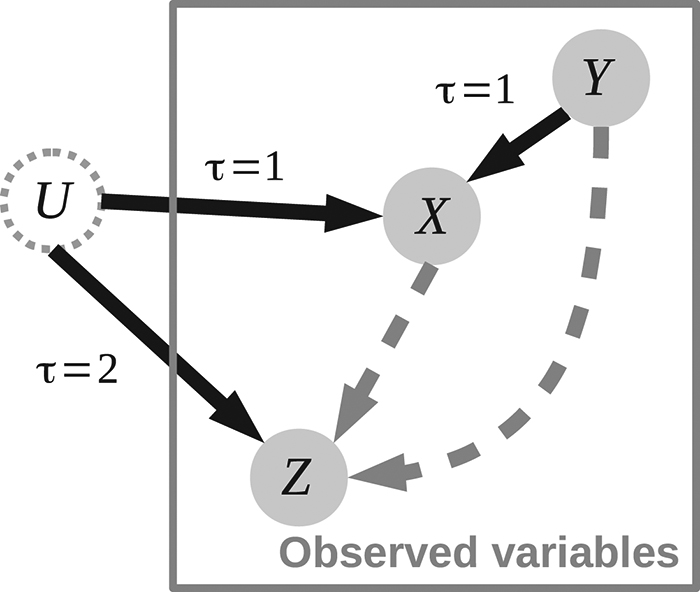
\includegraphics[width=0.2\textwidth]{img/causalsuff.jpeg}
    \caption{Example where Cusal Sufficency does not hold}
    \label{fig:causalsuff}
\end{figure}
Causal Sufficency is not always true, as we can see in Figure \ref{fig:causalsuff}, there if we dont't
observe the spurious variable $U$ we have that $Z$ depends on all the varibles (namely $X$ and $Y$).

\subsubsection*{Causal Markov Condition}
\begin{tcolorbox}[colback=red!5!white,colframe=red!75!black,title=\textbf{Separation Definition}]
    Two nodes $A$ and $B$ are separated given a conditioning set $S \text{ with } A, B \notin S$ 
    ($S$ may also be empty) if all paths between $A$ and $B$ are blocked, denoted:
    $A\bowtie B|S$.
\end{tcolorbox}
This simply means that a path is blocked if no link is available between two variables.
An example can be found in Figure \ref{fig:causalgraph}C where $X^1_t$ and $X^4_{t-1}$ have the path blocked.
\begin{tcolorbox}[colback=red!5!white,colframe=red!75!black,title=\textbf{Cusal Markov condition Definition}]
    The joint distribution of a time series process $\bm{X}$ with
    graph $G$ fulfills the Causal Markov Condition if and only if
    for all $Y_t\in \bm{X}_t$ with parents $\mathcal{P}_{Y_t}$ in the graph\\
    \begin{equation*}
        \bm{X}^-_t\setminus\mathcal{P}_{Y_t}\bowtie Y_t | \mathcal{P}_{Y_t}\implies\bm{X}^-_t\setminus\mathcal{P}_{Y_t}\Perp Y_t | \mathcal{P}_{Y_t}
    \end{equation*}
    that is, from separation in the graph (since the parents $\mathcal{P}_{Y_t}$ separate$Y_t$ from $\bm{X}^-_t\setminus\mathcal{P}_{Y_t}$ in the graph) follows indipendence.
\end{tcolorbox}
This definition simply means that if there is no path between two variables those are indipendent (indicated with the symbol $\Perp$) or said differently if we know $\mathcal{P}_{Y_t}$ (parents of $Y_t$) no other variable influences $Y_t$.
From this definition easily follows that Separation implies indipendence.

\subsubsection*{Faithfulness}
\begin{tcolorbox}[colback=red!5!white,colframe=red!75!black,title=\textbf{Faithfulness Definition}]
    The joint distribution of a time series process $\bm{X}$ with
    graph $G$ fulfills the Faithfulness condition if and only if for all
    disjoint subsets of nodes (or single nodes) $A, B, S \subset\mathcal{G}$ it
    holds that
    \begin{equation*}
        X_a \Perp X_b|X_S\implies A\bowtie B|S
    \end{equation*}
    that is, from independence follows separation, which includes its logical contraposition
    \begin{equation*}
        A\cancel{\bowtie} B|S\implies X_a \cancel{\Perp} X_b|X_S
    \end{equation*}
    from connectedness follows dependence.
\end{tcolorbox}
This definition states that from Indipendence follows Separation.

Intuitively, Faithfulness together with the Causal Markov Condition 
allow us to conclude that a measured
statistical dependency is actually due to some causal mechanism and, conversely,
a measured independence implies that no direct causal mechanism exists.
Both conditions are an important assumption for causal discovery algorithms that we'll discuss later.

\subsubsection*{Causal Stationarity}
\begin{tcolorbox}[colback=red!5!white,colframe=red!75!black,title=\textbf{Definition}]
    The time series process $\bm{X}$ with graph defined in \ref{fig:causalgraph}C is called causally stationary 
    over a time index set $\mathcal{T}$ if and only if for all links $X^i_{t-\tau}\rightarrow X^j_\tau$ in the graph
    \begin{equation*}
        X^i_{t-\tau}\cancel{\Perp}X^j_\tau|\bm{X}^-\setminus\{X^i_{t-\tau}\}\text{ holds for all } t\in\mathcal{T}
    \end{equation*}
\end{tcolorbox}
This constitutes actually a weaker form of stationarity than the common definition of stationarity in mean, 
variance, spectral properties, or of the value of individual coefficients in a linear model.
Intuitively this definition states that if I find a causal relation this should be time indipendent.\\

A typical reason for non-stationarity are confounder variables, i.e., wrong assumption in causal sufficiency.

\subsubsection*{Dependency (functional) type}
To test conditional independence hypotheses $X \Perp Y \;|\; Z$ different test statistics can be utilized.
These are typically based on making certain assumptions about the type of the underlying dependency structure.
While classical statistical methods are often based on the assumption of linearity (which
allows us to derive rigorous results), modern statistics, the physics community, and the recent 
field of machine learn-ing have developed non-parametric or model-free methods that allow us to better 
capture the nonlinear reality of many dynamical complex systems—at the cost of weaker theoretical results.
Conditional independence testing can be classified into regression-based and model-free approaches.\\
\begin{itemize}
    \item \textbf{Regression Based}: Regression-based conditional independence tests of $X\Perp Y\;|\;Z$ are based on 
    first regressing out the influence of Z from X and Y and then testing the dependence between the residuals.\\
    We first fit a model assuming:
    \begin{eqnarray*}
        X=f_X(Z)+\epsilon_X\\
        Y=f_Y(Z)+\epsilon_Y
    \end{eqnarray*}
    for centered variables $X, Y$ and independent and identicallynormally distributed $\epsilon_{X,Y}$.
    Secondly, from the estimated functions $\hat{f}$, the residuals are formed as
    \begin{eqnarray*}
        r_X=X-\hat{f}_X(Z)\\
        r_Y=Y-\hat{f}_Y(Z)
    \end{eqnarray*}
    Finally, the dependence between the residuals can be tested with different pairwise association tests (e.g., t-test).\\
    \item{\textbf{Model Free}}: model-free methods directly test conditional independence.
\end{itemize}

\begin{figure}[H]
    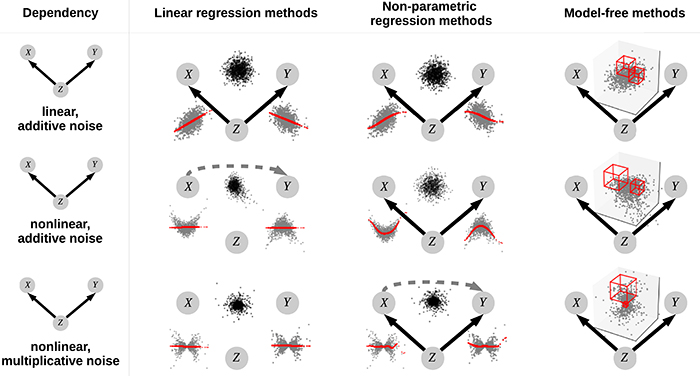
\includegraphics[width=0.9\textwidth]{img/depfunc.jpeg}
    \centering
    \caption{Illustration of applicability of different conditional independence methods(linear and non-parametric
    regression-based and model-free) on different types of linear and nonlinear common driver models. Black arrows 
    denote correctly identified causal links and dashed gray arrows indicate spurious links. The gray scatterplots 
    with red fit line illustrate regressions of X and Y on Z and the black scatterplot the dependency between the 
    residuals $r_X,r_Y$. The three-dimensional scatterplot with red cubes in the right column depicts the CMIknn test 
    which is based on data-adaptive nearest-neighbor estimation (the cubes are smaller for denser regions).}
\end{figure}

Model-free regression generally works, but they are very data-hungry and computationally expensive.

\subsection{Causal Discovery Algorithms}
\begin{tcolorbox}[colback=red!5!white,colframe=red!75!black,title=\textbf{Universal causal consistency Definition}]
Denoted by $\mathcal{\hat{G}}_n$ the estimated graph of some causal estimator from a sample of a 
distribution $P$ with sample size $n$ and by $\mathcal{G}$ the true causal graph. 
Then a causal estimator is said to be universally consistent if $\hat{\mathcal{G}}_n$ 
converges in probability to $\mathcal{G}$ for every distribution $P$,
\begin{equation*}
    \lim_{n\rightarrow\infty} Pr(\hat{\mathcal{G}}_n\ne\mathcal{G})=0
\end{equation*}
\end{tcolorbox}
Consistency is an important property of causal methods that tells us whether the method provably 
converges to the true causal graph in the limit of infinite sample size. That is, the probability of estimating 
the wrong graph becomes arbitrarily small if enough data is available, for any distribution $P$ (hence “universal”).

\subsubsection{FullCI Algorithm}
This is the simples algorithm that one can come up with, it tests for conditional independence between each
$X^i_{t-\tau}$ and $X^j_t$ conditioned on the entire past $\bm{X}_t^{(t-1,\;\ldots\;, t-\tau_{max})}$ excluding $X^i_{t-\tau}$.
\begin{equation}
    I^{FullCI}_{i\rightarrow j}(\tau)=I(X^i_{t-\tau};X_t^j|\bm{X}_t^{(t-1,\;\ldots\;, t-\tau_{max})}\setminus\{X^i_{t-\tau}\})
\end{equation}
This approach strongly suffers from the curse of dimensionality.
Complexity depends on the functional dependency assumption, assuming Linear dependency the complexity is
$\mathcal{O}(n(N\tau_{max})^2)$, where $N$ is the number of variables and $n$ is the sample size.

\subsection{Optimal Causation Entropy (OCE)}
A discovery algorithm based on the information-theoretic optimal causation entropy principle which reconstructs 
the lagged parents of a variable $X_t^j$ by an \textbf{iterative} procedure alleviating the curse of dimensionality.
Evaluates CMI \& Mutual Information (MI) in a forward-backward scheme for each variable.

\begin{equation}
    I(X;Y)=\int_Y\int_X{p(x,y)\log_2{\frac{p(x, y)}{p_1(x)p_2(y)}}dx\;dy}
\end{equation}
\begin{itemize}
    \item Forward: populate causal parents $\mathcal{P}^{OCE}(X^j_t)=\emptyset$
        \begin{itemize}
            \item 1st parent $\leftarrow$ maximize $I(X^i_{t-\tau};X^j_{t})$ for all $X^i_{t-\tau}\in\bm{X}_t^-$
            \item 2nd parent $\leftarrow$ maximize CMI $I(X^i_{t-\tau};X^j_{t}|X^{(1)})$
            \item 3rd parent $\leftarrow$ maximize CMI $I(X^i_{t-\tau};X^j_{t}|X^{(1)},X^{(2)})$
            \item $\ldots$ until CMI is significant (e.g., with t-test or non-linear methods) at each step we condition on all previous parents
        \end{itemize}
    \item Backward: prune not significant parents
    \begin{equation*}
        X^i_{t-\tau}\Perp X^j_{t} \;|\; \hat{\mathcal{P}}^{OCE}(X^j_t)\setminus\{X^i_{t-\tau}\}\quad
        \forall X^i_{t-\tau}\in\hat{\mathcal{P}}^{OCE}(X^j_t)
    \end{equation*}
    This means if the variable ($X^j_{t}$) is conditionally indipendent of a parent ($X^i_{t-\tau}$) given all the other parents
    excluded the parent we are evaluating ($\hat{\mathcal{P}}^{OCE}(X^j_t)\setminus\{X^i_{t-\tau}\}$) we can remove $X^i_{t-\tau}$
\end{itemize}

This algorithm has two main \textbf{\textcolor{Green}{advantages}}:
\begin{itemize}
    \item It is not necessary to condition on all variables and on all times
    \item The complexity is polynomial
\end{itemize}
While the main \textbf{\textcolor{Red}{drawback}} is that useless parents are added.

\end{document}